\documentclass[lang=cn,11pt,a4paper,cite=authornum]{paper}

\title{大数据技术基础 实验二 \\ 实验报告}
\author{毛子恒 \\ 2019211397}
\institute{北京邮电大学\ 计算机学院}

\date{\zhtoday}

% 本文档命令
\nocite{*}

\begin{document}

\maketitle

\section{概述}

\subsection{实验目的}

\begin{enumerate}
    \item 了解IDEA构建大数据工程的过程
    \item 熟悉使用Java语言编写大数据程序;
    \item 了解 MapReduce 的工作原理;
    \item 掌握在集群上运行程序的方法。
\end{enumerate}

\subsection{实验步骤}

\begin{enumerate}
    \item 使用IDEA构建大数据工程;
    \item 编写WordCount程序;
    \item 程序打包和运行。
\end{enumerate}

\section{实验结果及分析}

\paragraph{WordCount程序}

依照指导书编写WordCount程序。

\mintinline{text}{WordCount}是实现通过MapReduce统计单词数量的类,其中包含两个子类\mintinline{text}{TokenizerMapper}和\mintinline{text}{IntSumReducer},分别实现了Map和Reduce过程。

\mintinline{text}{TokenizerMapper}类如\figref{fig:map}所示,该类的\mintinline{text}{map}方法用于将输入转化为形如\mintinline{text}{{word: 1}}的键值对。

\begin{figure}[!htb]
    \centering
    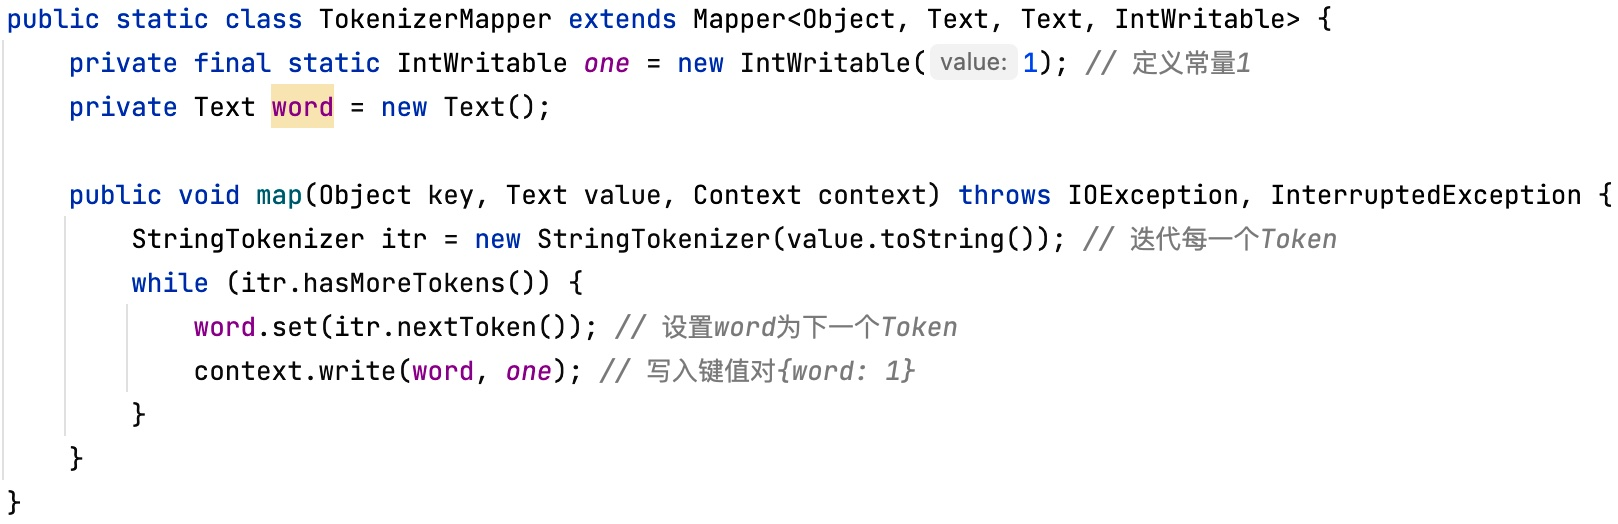
\includegraphics[width=\textwidth]{./images/map.jpg}
    \caption{TokenizerMapper类\label{fig:map}}
\end{figure}

\mintinline{text}{IntSumReducer}类如\figref{fig:reduce}所示,该类用于将具有相同键的各个值求和,统计出各个单词出现的次数,转化为形如\mintinline{text}{{word: 2}}的键值对。

\begin{figure}[!htb]
    \centering
    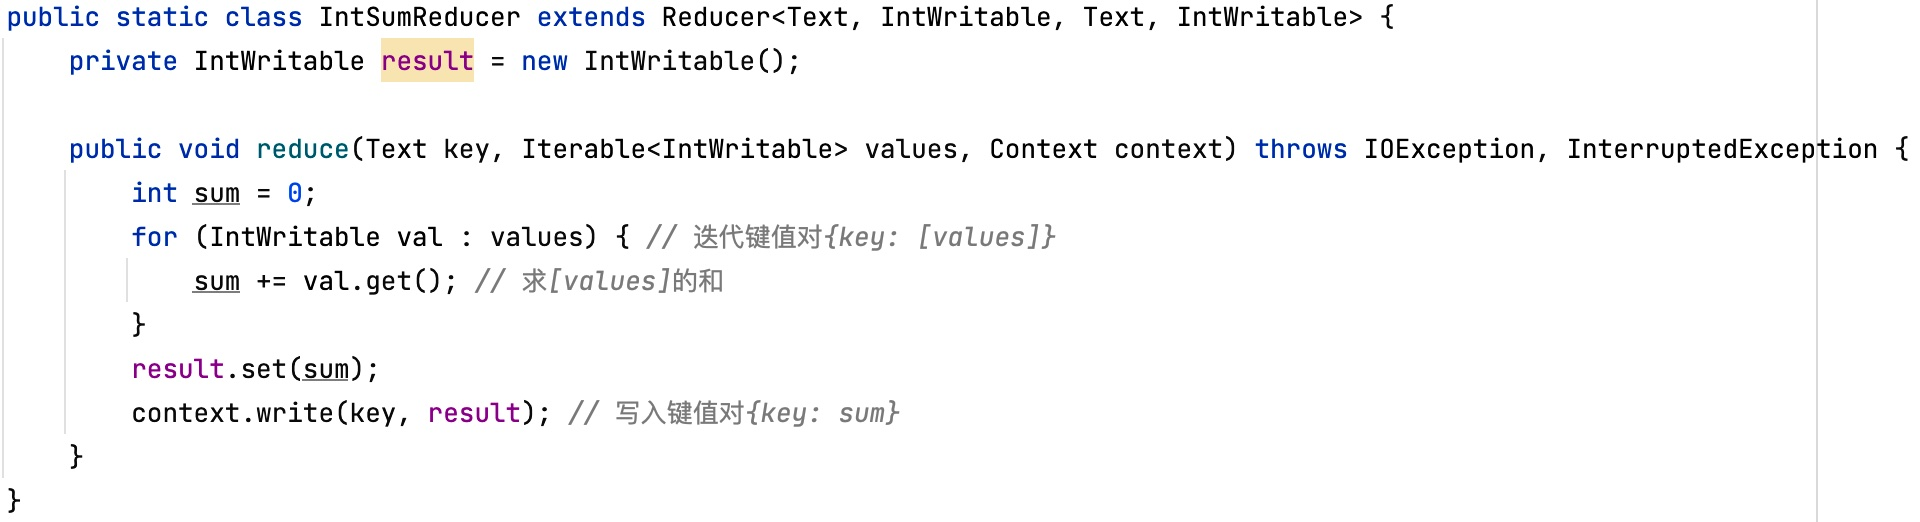
\includegraphics[width=\textwidth]{./images/reduce.jpg}
    \caption{IntSumReducer类\label{fig:reduce}}
\end{figure}

\mintinline{text}{WordCount}类的\mintinline{text}{main}方法如\figref{fig:main}所示,该方法是程序的入口,用于获取系统配置、输入输出路径、装载类以及驱动job进行。

\begin{figure}[!htb]
    \centering
    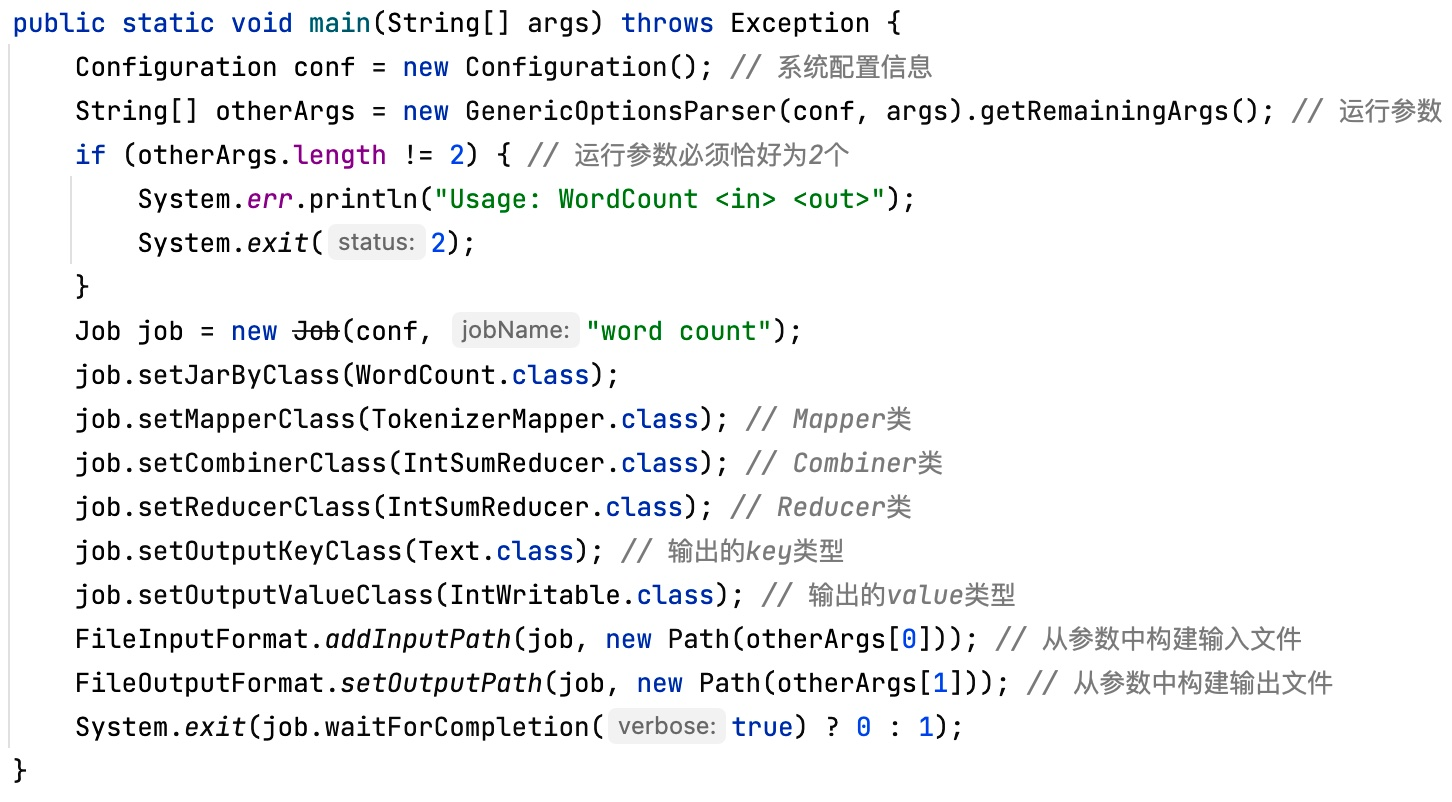
\includegraphics[width=0.9\textwidth]{./images/main.jpg}
    \caption{main方法\label{fig:main}}
\end{figure}

\paragraph{程序打包}

依照指导书的说明打包生成jar包,如\figref{fig:jar},去除其中的MANIFEST.MF文件,并且上传到服务器。

\begin{figure}[!htb]
    \centering
    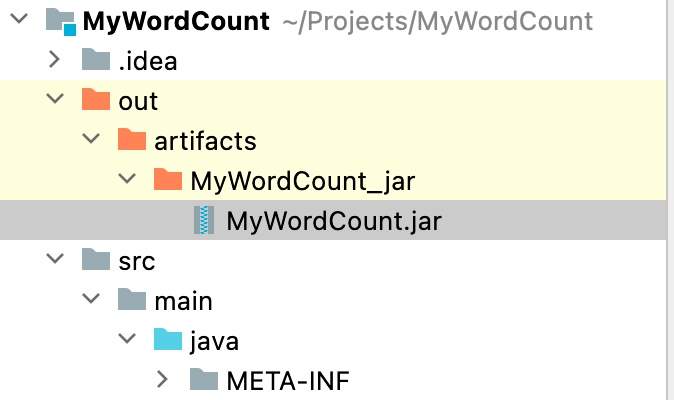
\includegraphics[width=0.4\textwidth]{./images/jar.jpg}
    \caption{程序打包\label{fig:jar}}
\end{figure}

\paragraph{程序运行}

首先创建输入文件\mintinline{text}{2019211397-mzh-input.txt},内容如\figref{fig:input}。

\begin{figure}[!htb]
    \centering
    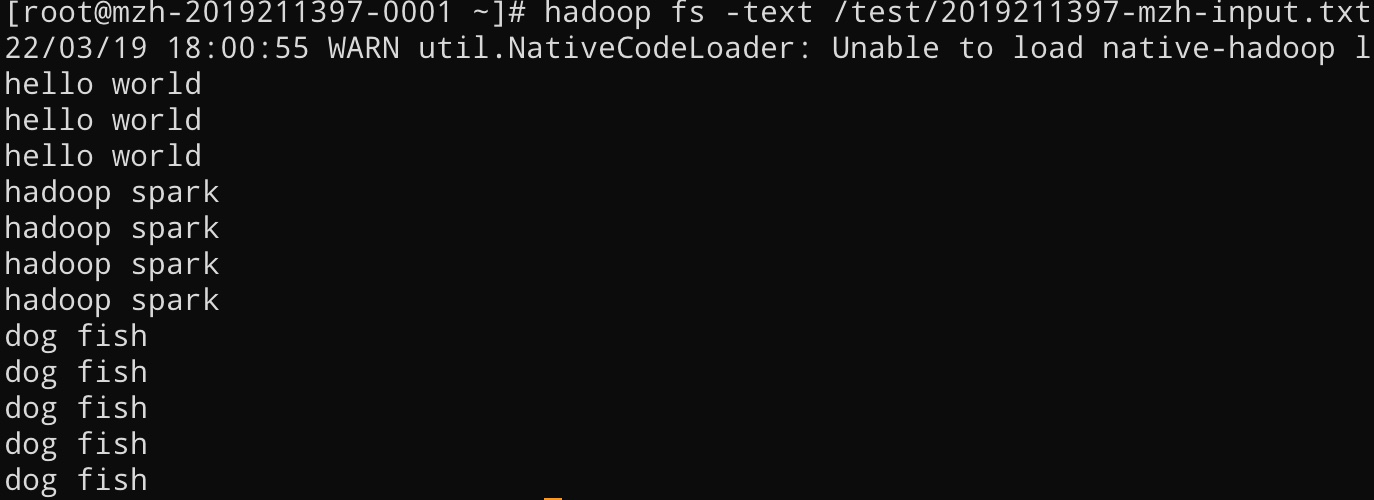
\includegraphics[width=0.7\textwidth]{./images/input.jpg}
    \caption{输入文件\label{fig:input}}
\end{figure}

启动集群,通过如下命令创建文件夹并且将输入文件传入HDFS当中:

\begin{code}
\begin{minted}{shell}
hadoop fs -mkdir -p /test
hadoop fs -put ./2019211397-mzh-input.txt /test/2019211397-mzh-input.txt
\end{minted}
\end{code}

在此处如果出现“There are 0 datanode(s) running and no node(s) are excluded in this operation.”的错误,那么应该检查DataNode是否已经启动,首先停止集群,检查四个主机的core-site.xml中的\mintinline{text}{hadoop.tmp.dir}项应该为\mintinline{text}{/home/modules/hadoop-2.7.7/tmp},同时删除各个主机下的这个文件夹,并且注释hosts文件中127.0.0.1的有关项,最后重新启动集群。

运行命令和结果如\figref{fig:job}和\figref{fig:res}所示,可见利用打包好的jar包中的WordCount类,我们成功发起并完成了一个mapreduce的job。

\begin{figure}[!htb]
    \centering
    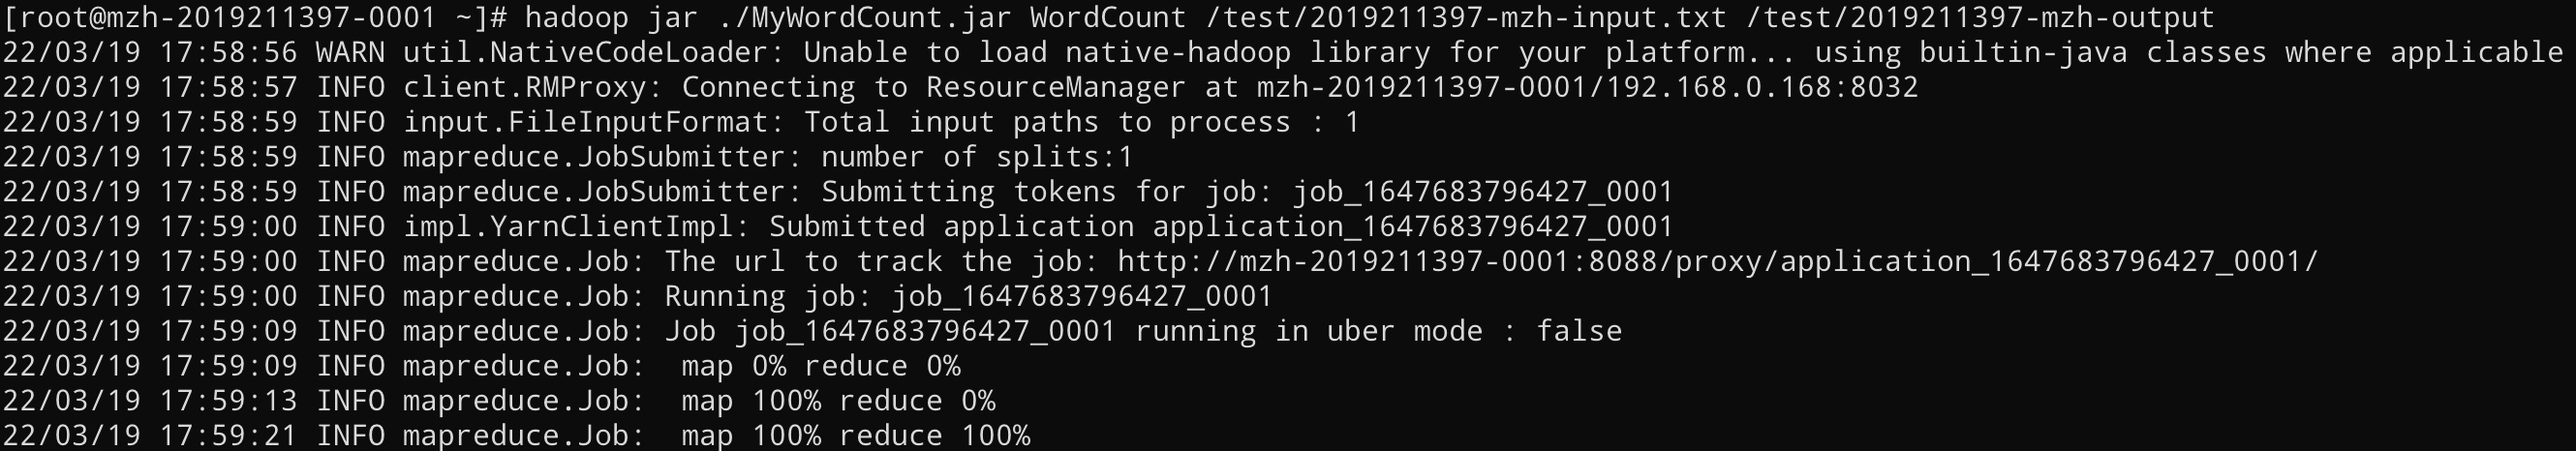
\includegraphics[width=\textwidth]{./images/job.jpg}
    \caption{运行命令\label{fig:job}}
\end{figure}

\begin{figure}[!htb]
    \centering
    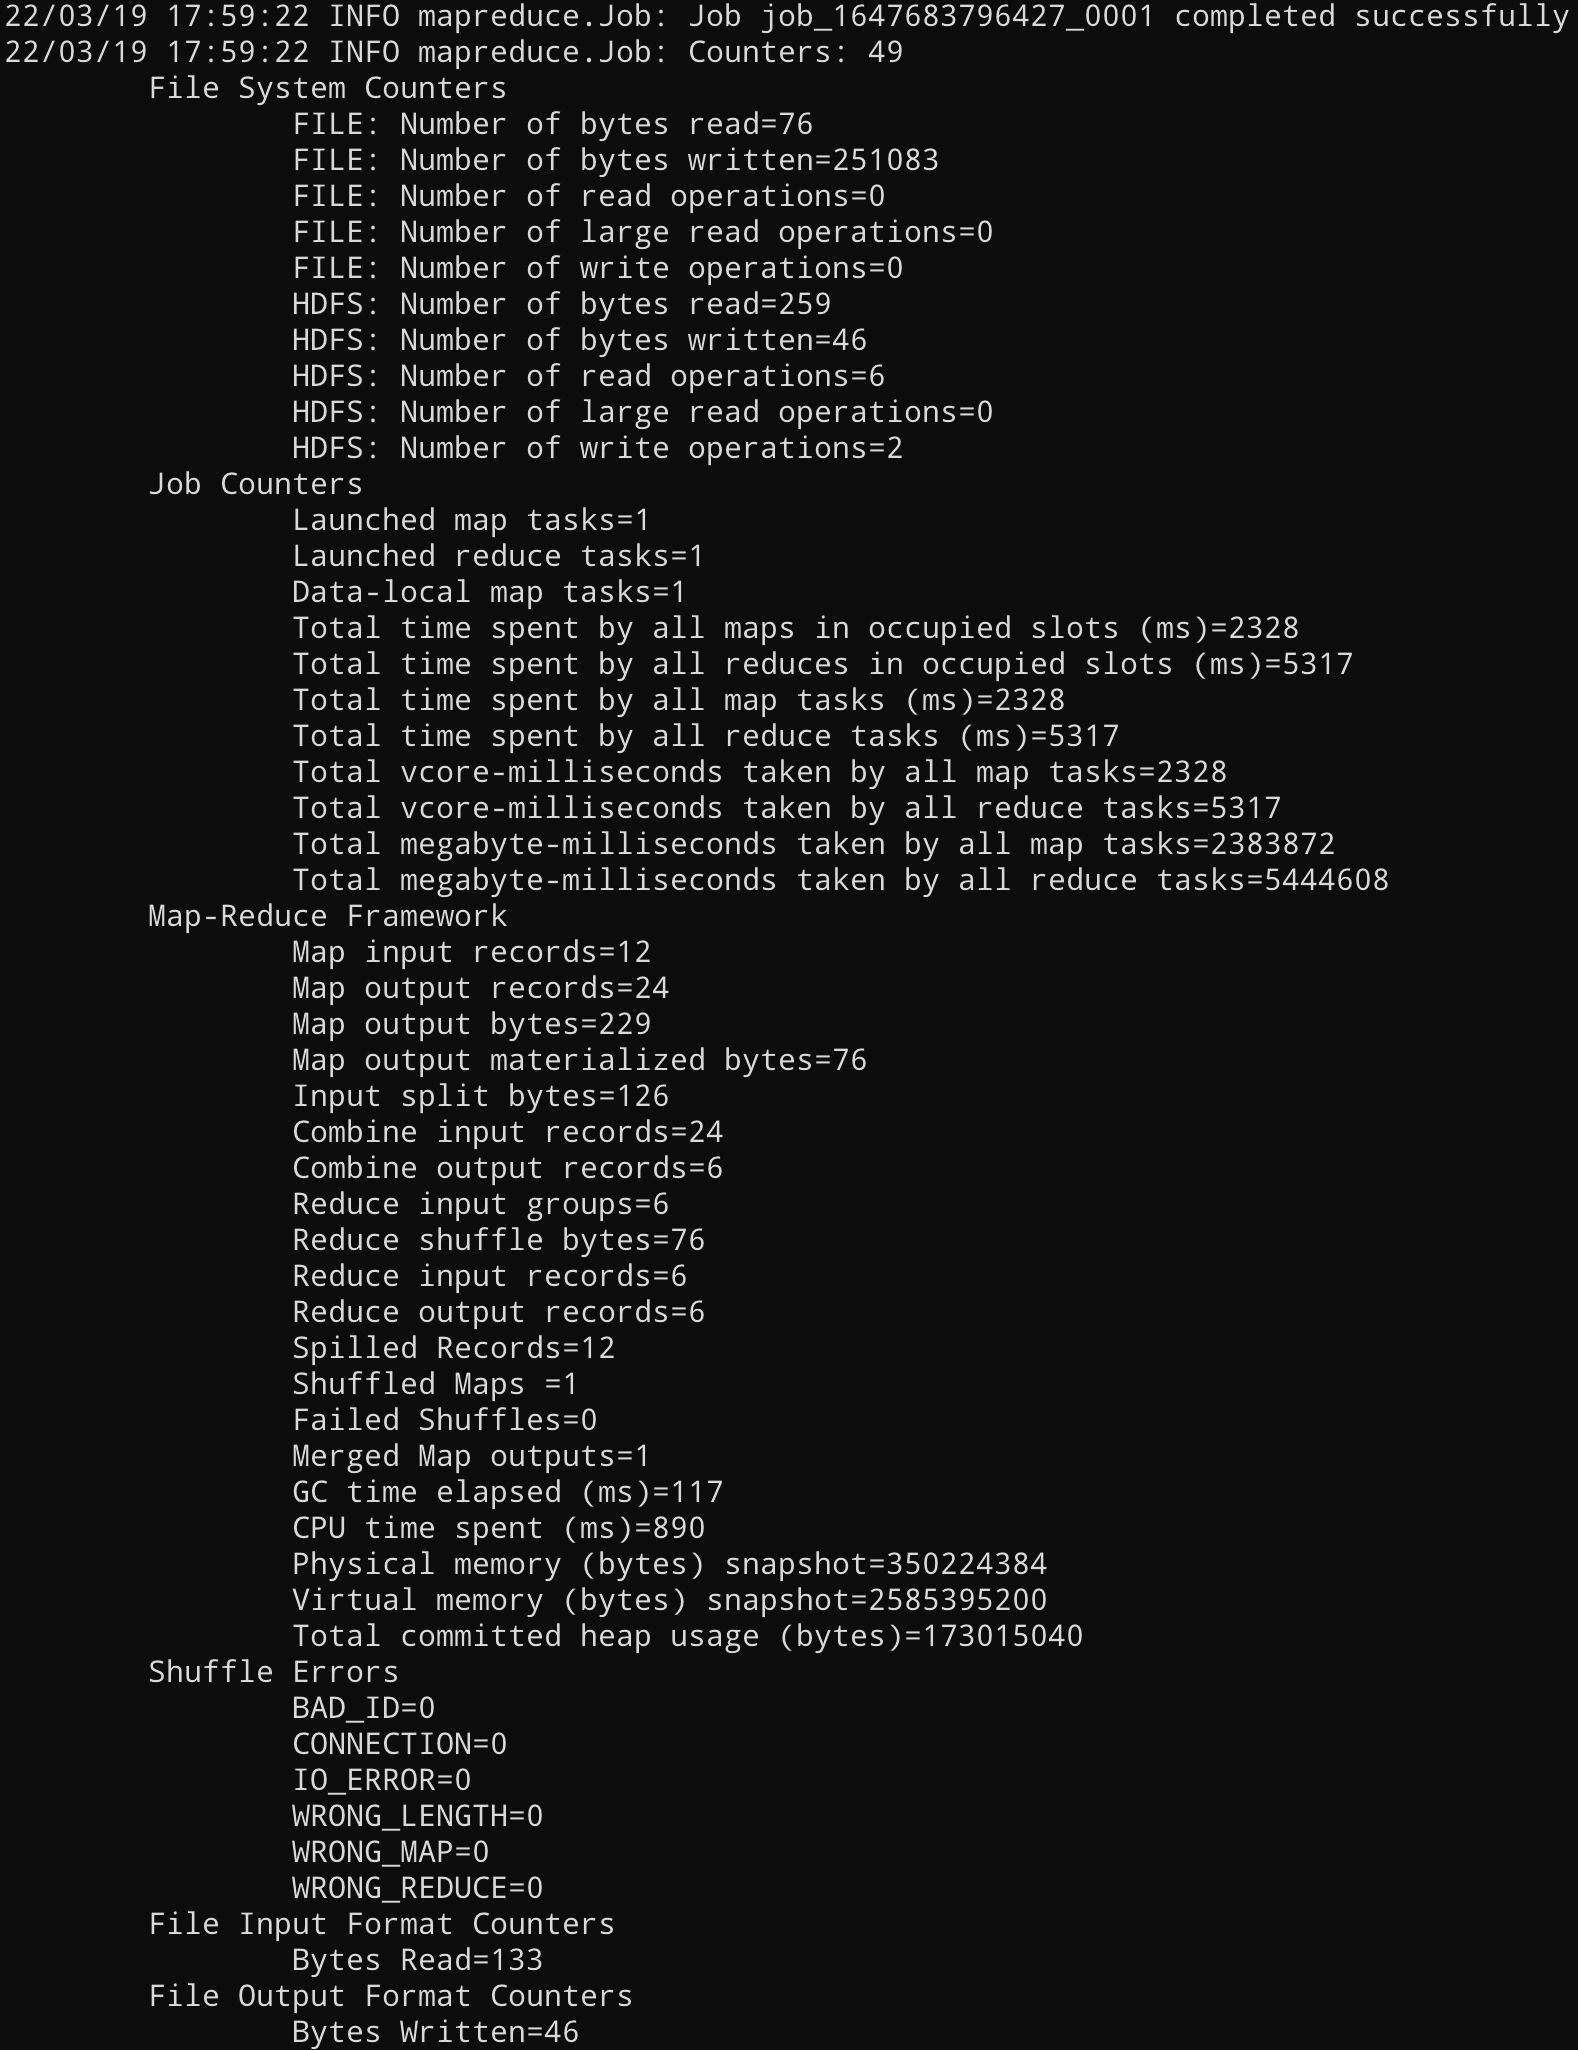
\includegraphics[width=0.8\textwidth]{./images/res.jpg}
    \caption{运行结果\label{fig:res}}
\end{figure}

最后得到的统计结果如\figref{fig:output}所示。

\begin{figure}[!htb]
    \centering
    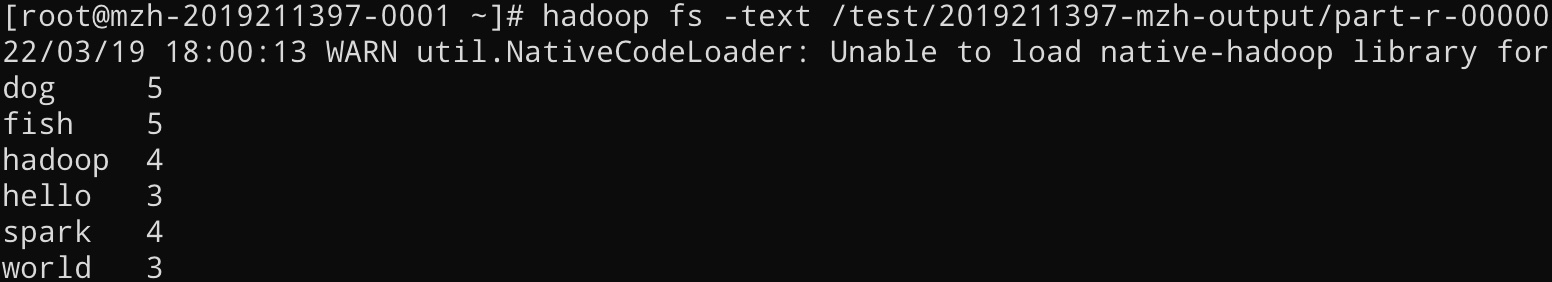
\includegraphics[width=0.7\textwidth]{./images/output.jpg}
    \caption{输出文件\label{fig:output}}
\end{figure}

\section{实验总结}

本次实验中我编写代码进行了简单的MapReduce操作,使我的Java代码能力得到了增强,对HDFS和MapReduce的原理理解更加深刻。

\end{document}
